%% For double-blind review submission, w/o CCS and ACM Reference (max submission space)
\documentclass[acmsmall,review,anonymous]{acmart}\settopmatter{printfolios=true,printccs=false,printacmref=false}
%% For double-blind review submission, w/ CCS and ACM Reference
%\documentclass[acmsmall,review,anonymous]{acmart}\settopmatter{printfolios=true}
%% For single-blind review submission, w/o CCS and ACM Reference (max submission space)
%\documentclass[acmsmall,review]{acmart}\settopmatter{printfolios=true,printccs=false,printacmref=false}
%% For single-blind review submission, w/ CCS and ACM Reference
%\documentclass[acmsmall,review]{acmart}\settopmatter{printfolios=true}
%% For final camera-ready submission, w/ required CCS and ACM Reference
%\documentclass[acmsmall]{acmart}\settopmatter{}
\usepackage{algorithm,algorithmic}
%\usepackage{xcolor}

\newcommand{\TODO}[1]{({\bf{{TODO:}}}\,\,\,{\footnotesize\it{#1}})}

%% Journal information
%% Supplied to authors by publisher for camera-ready submission;
%% use defaults for review submission.
\acmJournal{PACMPL}
\acmVolume{1}
\acmNumber{CONF} % CONF = POPL or ICFP or OOPSLA
\acmArticle{1}
\acmYear{2018}
\acmMonth{1}
\acmDOI{} % \acmDOI{10.1145/nnnnnnn.nnnnnnn}
\startPage{1}

%% Copyright information
%% Supplied to authors (based on authors' rights management selection;
%% see authors.acm.org) by publisher for camera-ready submission;
%% use 'none' for review submission.
\setcopyright{none}
%\setcopyright{acmcopyright}
%\setcopyright{acmlicensed}
%\setcopyright{rightsretained}
%\copyrightyear{2018}           %% If different from \acmYear

%% Bibliography style
\bibliographystyle{ACM-Reference-Format}
%% Citation style
%% Note: author/year citations are required for papers published as an
%% issue of PACMPL.
\citestyle{acmauthoryear}   %% For author/year citations


%%%%%%%%%%%%%%%%%%%%%%%%%%%%%%%%%%%%%%%%%%%%%%%%%%%%%%%%%%%%%%%%%%%%%%
%% Note: Authors migrating a paper from PACMPL format to traditional
%% SIGPLAN proceedings format must update the '\documentclass' and
%% topmatter commands above; see 'acmart-sigplanproc-template.tex'.
%%%%%%%%%%%%%%%%%%%%%%%%%%%%%%%%%%%%%%%%%%%%%%%%%%%%%%%%%%%%%%%%%%%%%%


%% Some recommended packages.
\usepackage{booktabs}   %% For formal tables:
                        %% http://ctan.org/pkg/booktabs
\usepackage{subcaption} %% For complex figures with subfigures/subcaptions
                        %% http://ctan.org/pkg/subcaption


\begin{document}

%% Title information
\title[Short Title]{Full Title}         %% [Short Title] is optional;
                                        %% when present, will be used in
                                        %% header instead of Full Title.
\titlenote{with title note}             %% \titlenote is optional;
                                        %% can be repeated if necessary;
                                        %% contents suppressed with 'anonymous'
\subtitle{Subtitle}                     %% \subtitle is optional
\subtitlenote{with subtitle note}       %% \subtitlenote is optional;
                                        %% can be repeated if necessary;
                                        %% contents suppressed with 'anonymous'


%% Author information
%% Contents and number of authors suppressed with 'anonymous'.
%% Each author should be introduced by \author, followed by
%% \authornote (optional), \orcid (optional), \affiliation, and
%% \email.
%% An author may have multiple affiliations and/or emails; repeat the
%% appropriate command.
%% Many elements are not rendered, but should be provided for metadata
%% extraction tools.

%% Author with single affiliation.
\author{First1 Last1}
\authornote{with author1 note}          %% \authornote is optional;
                                        %% can be repeated if necessary
\orcid{nnnn-nnnn-nnnn-nnnn}             %% \orcid is optional
\affiliation{
  \position{Position1}
  \department{Department1}              %% \department is recommended
  \institution{Institution1}            %% \institution is required
  \streetaddress{Street1 Address1}
  \city{City1}
  \state{State1}
  \postcode{Post-Code1}
  \country{Country1}                    %% \country is recommended
}
\email{first1.last1@inst1.edu}          %% \email is recommended

%% Author with two affiliations and emails.
\author{First2 Last2}
\authornote{with author2 note}          %% \authornote is optional;
                                        %% can be repeated if necessary
\orcid{nnnn-nnnn-nnnn-nnnn}             %% \orcid is optional
\affiliation{
  \position{Position2a}
  \department{Department2a}             %% \department is recommended
  \institution{Institution2a}           %% \institution is required
  \streetaddress{Street2a Address2a}
  \city{City2a}
  \state{State2a}
  \postcode{Post-Code2a}
  \country{Country2a}                   %% \country is recommended
}
\email{first2.last2@inst2a.com}         %% \email is recommended
\affiliation{
  \position{Position2b}
  \department{Department2b}             %% \department is recommended
  \institution{Institution2b}           %% \institution is required
  \streetaddress{Street3b Address2b}
  \city{City2b}
  \state{State2b}
  \postcode{Post-Code2b}
  \country{Country2b}                   %% \country is recommended
}
\email{first2.last2@inst2b.org}         %% \email is recommended


%% Abstract
%% Note: \begin{abstract}...\end{abstract} environment must come
%% before \maketitle command
\begin{abstract}
Text of abstract \ldots.
\end{abstract}


%% 2012 ACM Computing Classification System (CSS) concepts
%% Generate at 'http://dl.acm.org/ccs/ccs.cfm'.
\begin{CCSXML}
<ccs2012>
<concept>
<concept_id>10011007.10011006.10011008</concept_id>
<concept_desc>Software and its engineering~General programming languages</concept_desc>
<concept_significance>500</concept_significance>
</concept>
<concept>
<concept_id>10003456.10003457.10003521.10003525</concept_id>
<concept_desc>Social and professional topics~History of programming languages</concept_desc>
<concept_significance>300</concept_significance>
</concept>
</ccs2012>
\end{CCSXML}

\ccsdesc[500]{Software and its engineering~General programming languages}
\ccsdesc[300]{Social and professional topics~History of programming languages}
%% End of generated code


%% Keywords
%% comma separated list
\keywords{Allscale API, parallel computing, modelling}  %% \keywords are mandatory in final camera-ready submission


%% \maketitle
%% Note: \maketitle command must come after title commands, author
%% commands, abstract environment, Computing Classification System
%% environment and commands, and keywords command.
\maketitle


\section{Introduction}

Text of paper \ldots

\section{Problem formulation}

In this paper, the capabilities of Allscale API will be demonstrated by modelling how contaminating substance spread over in marine environment or any other open space. Suppose at time $t=0$ and some point ${\bf p}_c$ of rectangular domain $\Omega$ a contaminating substance had been spilled out with high concentration. Neither position ${\bf p}_c$ nor the initial concentration level are known in advance. However, we can monitor the situation at few sensors randomly seeded inside the domain, see example on Fig~\ref{fig:sensors}. The sensors are assumed sufficiently accurate but scarce in number.

The physical model of such a process is well studied and mathematically characterized by advection-diffusion partial differential equation (PDE), which describes physical phenomena where quantities are transferred inside a system due to advection and diffusion. For the full treatment of this class of PDE, reader is referred to \cite{Hundsdorfer03}.

Implying the marine environment (as an example) and assuming that we can (1) measure the concentration of contaminant at sensor locations; (2) measure the speed and direction of the current at sensor locations; and (3) we know the diffusion coefficient $D$ for contaminant in the saline water; the \textit{data assimilation} problem, we are going to solve, can be formulated as follow: \textit{find a reasonably good approximation to the distribution of contaminant in the domain as a function of space and time given only a physical model and sensor observations (concentration and flow velocity)}.

\begin{figure}
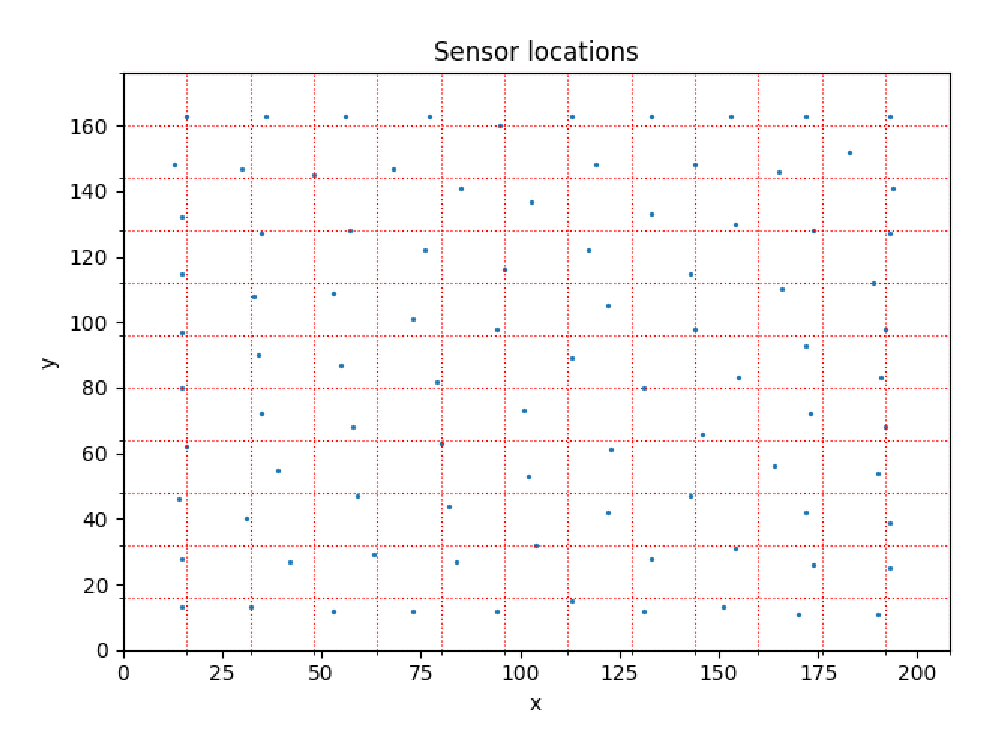
\includegraphics[scale=0.5]{images/sensors-Nx208-Ny176}
\caption{Example of domain decomposition into ${16{\times}16}$ cells. Blue points depict location of sensors pseudo-randomly scattered across the domain. Coordinates are defined as indices of nodal points.}
\label{fig:sensors}
\end{figure}

\subsection{Top level view of the method}

Since our main goal is to demonstrate the power of Allscale API in application to the real problems, we would like to depart from for-now-inessential details such as data acquisition from the physical sensor devices, data storage format, etc., assuming that exploration engineers always know how to cope with these things. Instead, the \textit{simulated data} will be generated and used for simplicity. The advantage of having a ``ground-truth'' is that it can be compared against the data assimilation solution for the assessment of method's accuracy.

In reality the ground-truth density field $u_{gt}(x,y,t)$, which we simulate directly here, is never available. At every time step we extract and record the values of $u_{gt}(x,y,t)$ at few sensor locations: $z_s(t)$ = $u_{gt}(x_s,y_s,t)$, $\,\,s \in [1\,{\ldots}\,N_{sensors}]$. The entities $\{z_s(t)\}$ are called \textit{observations} and this is the only information available to the data assimilation method about ``true state of nature''. The sensors themselves are pseudo-randomly scattered across the domain, Fig.~\ref{fig:sensors}, where the term ``pseudo-randomly'' means each sensor is neither too close nor too far from its nearest neighbours.

Over the course of time integration, we save $100$ snapshots of the entire ground-truth density field $u_{gt}(x,y,t)$ as well as data assimilation solution $u(x,y,t)$. By the end of simulation, these snapshots are used for comparison. The amount of stored data grows rapidly with the resolution, however, $100$ is quite affordable number in many cases.    

Essential feature of Allscale API is domain sub-division into so called \textit{cells}, Fig.~\ref{fig:sensors}. For now, we just accept that any computation is \textit{always} done over a cell (or a sub-domain) of the whole domain $\Omega$ almost independently of other sub-domains. We say ``almost'' because it is possible to exchange border point values with immediate neighbours, see Section~\ref{?} for details. 

We integrate forward in time over the period $[0 \ldots T]$ both --- the ground-truth and the data assimilation simulations. The data assimilation method starts from zero density $u(x,y,t)\rvert_{t=0} = 0$ pretending we do not know at which point contamination had happened. As the time integration progressing, non-zero field $u(x,y,t)$ emerges, which we believe estimates the ``true state of nature'' $u_{gt}(x,y,t)$ quite well. Let us now take the top level view. Algorithm~\ref{alg:toplevel} summarizes the major steps in the data assimilation method:

\begin{algorithm}[!htb]
\caption{Data Assimilation Framework}
\label{alg:toplevel}
\algsetup{indent=2em}
\begin{algorithmic}[1]
\STATE{\small\#\#\# \textit{$*****$ Generator of ground-truth and observations. $*****$}}
\STATE\textbf{Require}: generate ground-truth and observations, Section~\ref{?}:
{
    \STATE\hspace{2em}{create initial field $u_{gt}(x,y,t)\rvert_{t=0}$ =
                      $a\,\delta(x-x_c,y-y_c),\,\,\,\forall\,x,y\in\Omega$;}
    \STATE\hspace{2em}{generate a file of pseudo-randomly seeded sensor locations;}
    \STATE\hspace{2em}{integrate the governing equation (\ref{eq:pde}) forward in time
                      $t=0\!:\!T$;}
    \STATE\hspace{2em}{while integrating, write a file of observations
                      $\{z_s(t)\,|\,s=1\!:\!N_{sensors},\, t=0\!:\!T\}$;}
    \STATE\hspace{2em}{while integrating, store $100$ snapshots of $u_{gt}(x,y,t)$.}
}
\STATE{}
\STATE{\small\#\#\# \textit{$*****$ Data-assimilation solver. $*****$}}
\STATE\textbf{Input}: file of sensor locations, file of observations, 
      initial field $u(x,y,t)\rvert_{t=0} = 0,\,\,\,\forall\,x,y\in\Omega$.
\STATE{\textbf{Require}: sub-divide the whole domain $\Omega$ into a number of cells $N_{cells}$; this is automatically done by Allscale API.}
\STATE{\small\#\#\# \textit{Integrate forward in time and estimate the density field $u(x,y,t)$}.}
\FOR{\label{alg:line-outerloop}\,\,({\small with time-step $\Delta{t}$ (\ref{eq:time-step})})\,\,$t=0$ \TO $T$}
    \FOR{\label{alg:line-relax}$r=1$ \TO $N_{relaxations}$}
        \FOR{\,\,{\small(\textit{in parallel using Allscale API})}\,\, $c=1$ \TO $N_{cells}$}
            \IF{$c$-th cell contains at least one sensor}
            \STATE{\label{alg:line-kalman}Propagate state inside $c$-th cell using the Kalman filter and previously recorded observations $\{z_s(t)\}$, Section~\ref{sec:kalman}.}
            \ELSE
            \STATE{Reduce the time step: $\Delta{t}^* = \Delta{t}/N_{relaxations}$.}
            \STATE{\small\#\#\# \textit{Section~\ref{sec:finit-diff}, formula (\ref{eq:state-propag})}:}
            \STATE{\label{alg:line-conven}Solve governing equation forward in time (\ref{eq:pde}) inside $c$-th cell: ${\bf u}_{t+1} = {\bf B}^{-1}_t {\bf u}_{t}$.}
            \ENDIF
        \ENDFOR
    \ENDFOR
\STATE{while integrating, store $100$ snapshots of $u(x,y,t)$.}
\ENDFOR
\end{algorithmic}
\end{algorithm}

Some comments should be made at this point. Just integration forward in time does not make sense because the field $u(x,y,t)$ would remain zero unless observations are somehow utilized.
We employ Kalman filter (line~\ref{alg:line-kalman}) that brings otherwise zero density closer to observation (if there is a sensor in the cell), and this important driving force is responsible for convergence of estimated density field towards the true state. In the absence of observations in a cell, the conventional integration step is fulfilled (line~\ref{alg:line-conven}).

Each iteration in the outer loop (line~\ref{alg:line-outerloop}) is sub-divided into several smaller \textit{relaxation} steps called \textit{sub-iterations} (line~\ref{alg:line-relax}). The rationale is to exchange information between neighbouring cells, especially between those with and without observations. Recall, computation in each cell is done independently. We found that better overall consistency can achieved by improving Kalman filtering estimation through the additional relaxation process on each time-integration iteration. The number of sub-iterations $N_{relaxations}$ can be relatively small, typically 5 to 7 in our experiments. 

It is also worth to mention the \textit{multi-scaling} capability of Allscale API. Cells can be processed at different resolutions, and we simultaneously use the ones with $16{\times}16$ and $8{\times}8$ nodal points. Namely, the cells with observations are processed at fine resolution because this yields better Kalman filtering estimation. On the other hand, cells without observations (where we just integrate the governing equation) are processed at coarse resolution with less computational cost.

\subsection{Mathematical definition}

Advection-diffusion equation is widely used for process modelling in variety of problems. Reader can find many interesting references to the real world applications in \cite{Miyaoka17}.

In this study, we simulate propagation of contaminant in 2D (marine) environment where density is defined as a function of space and time $u$ = $u(x,y,t)$. The physical model of contaminant being dispersed and transported over a spacial domain is governed the following equation:
\begin{equation}
\frac{\partial u}{\partial t} =
D \left(\frac{\partial^2 u}{\partial x^2} + \frac{\partial^2 u}{\partial y^2}\right)
- v_x \frac{\partial u}{\partial x}
- v_y \frac{\partial u}{\partial y},
\,\,\,\,\,\,\mbox{s.t.}\,\,\,\,\,\,
u\rvert_{t=0} = a\,\delta(x\!-\!x_c,y\!-\!y_c),
\,\,\,\,\,\,u\rvert_{\partial\Omega}=0.
\label{eq:pde}
\end{equation}
where $D$ is a known diffusion coefficient, $v_x = v_x(x,y,t)$, $v_y = v_y(x,y,t)$ are the flow (current) velocity components, the initial condition is defined a ``one-shot'' contamination at some point $(x_c,y_c)$, and the boundary condition is of homogeneous Dirichlet type.

The scaling factor $a$ in (\ref{eq:pde}) defines the units of density function. Here we are mostly interested in how density is distributed in the space, i.e. the \textit{relative} level of concentration in different parts of the domain $\Omega$. As such, the scaling factor $a$ does not play an important role and can be set to any number of abstract ``units'' (we arbitrarily choose $a = 10^4$). However, in the concrete application, this factor must be set to a physically meaningful value, of course.

In fact, the entity $u(x,y,t)$ can describe very different phenomena. For example, it could be traffic density on city roads, the number per square kilometre of living creatures migrating in certain area and so on. Whatever phenomenon underlying the process in question, its important characteristic is the relative proportion of diffusion and advection. Namely, the process can be categorized as advection dominated, diffusion dominated or intermediate case. It turns out, the equation where advection dominates is harder to solve numerically \cite{Langtangen16}. On the other hand, the case of strong diffusion predomination is not quite interesting for presentation.

Non-dimensional \textit{Peclet} number \cite{Socolofsky05}, $Pe = D/(v_0^2 t)$, provides qualitative estimation of what might be a reasonable choice for the coefficient of diffusion $D$ and the absolute value of expected flow velocity $v_0$. In simulation we want visible presence of both advection and diffusion to show up. We set by default $D$ = $1\,[m^2/s]$ and $v_0$ = $1\,[m/s]$. At beginning $Pe = O(1)$ and diffusion is strong enough. As time grows, the advection term gradually overtakes the diffusion and $Pe$ becomes smaller $Pe \ll 1$.

Boundary condition is another important step in problem setup. Ideally, the absorbing boundary condition should be applied at the outer border $\partial\Omega$ of the domain $\Omega$. In our case, a high density value is mostly obtained far from the boundary and we can go for a simple Dirichlet condition. The paper \cite{Miyaoka17} gives valuable insight into various boundary condition cases pertain to advection-diffusion equation.

In next few sections we shall describe the numerical scheme used for problem discretization and time-integration of the governing PDE. Allscale API prescribes certain computational design as will be explained therein. 

\subsection{Grid of cells}

Allscale API offers two layers of domains discretization. At the top level, the whole domain is represented as a rectangular \textit{grid of cells}, and the number of cells is not limited in either dimension. The cells itself is implemented as a \textit{grid of nodal points}. The size of a cell must be fixed because it is defined by template parameters in corresponding \texttt{C++} class and should be available at compile time.

At the run time, each cell is assigned to so called \textit{worker} --- either an execution thread or a process in case of distributed application. The assignment and workload balancing is done automatically once the grid of cells had been exposed to \textit{parallel for} (\texttt{pfor}) or \texttt{stencil} operator. \TODO{section for stencil API, reference}

A portion of grid cell layout is exemplified on Fig.~\ref{fig:cell}. As it was already mentioned, computation over nodal points of each cell is conducted independently of other cell with no-race-condition guarantee when border points of four immediate peer cells are being read (green point on Fig.~\ref{fig:cell}). In contemporary implementation of \texttt{stencil} operator the two grids of cell are actually used --- the ``current'' one holds the state attained so far and the ``next'' one we update with the new state estimation. Once all the cells have finished, the grids are swapped and the process repeats on the next iteration.

\begin{figure}[!htb]
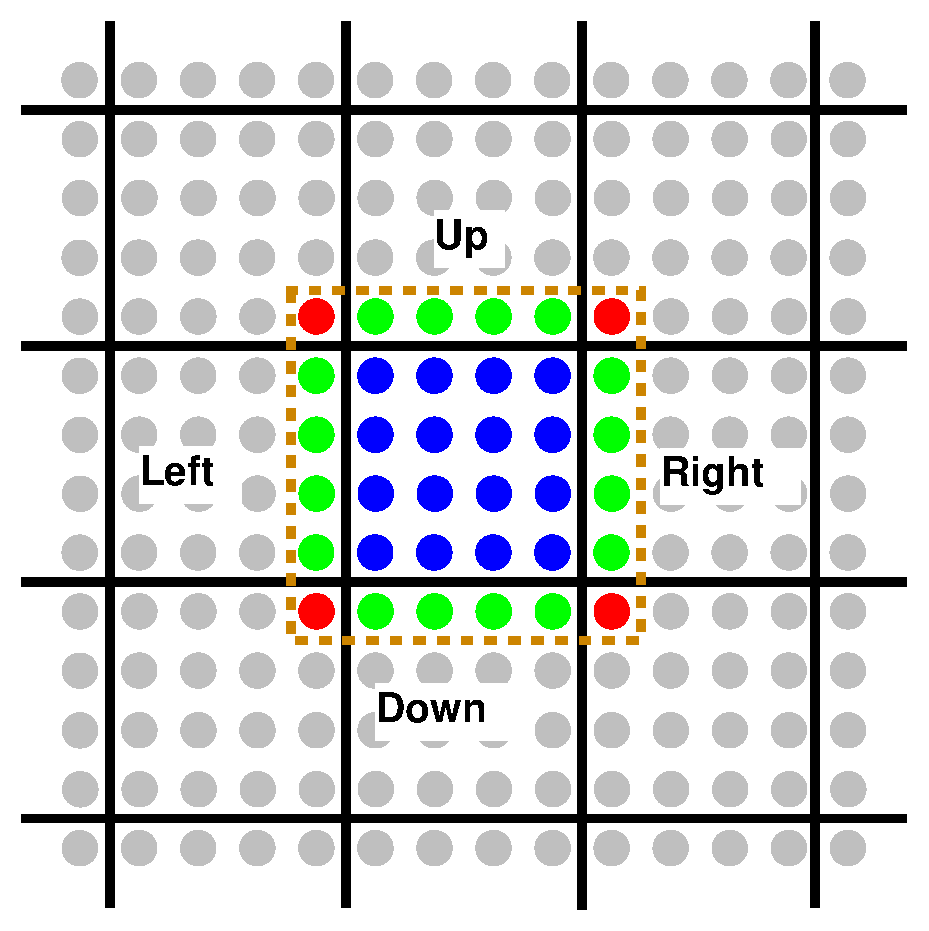
\includegraphics[scale=0.33]{images/subdomain.eps}
\caption{Example of a grid cell, constituted by the blue nodal points, and corresponding extended one, outlined by dotted rectangle. Border (green) points of four immediate peer cells (\textit{Left}, \textit{Right}, \textit{Up}, \textit{Down}) are available for exchange. Diagonal peer cells are unreachable as well as their (red) points.}
\label{fig:cell}
\end{figure}

In order to yield a seamless solution we operate over \textit{extended cell} that comprises border points of the peer cells. Extended cell is depicted by dotted rectangle on Fig.~\ref{fig:cell}. During computation, the corner nodal points (shown in red) are ignored because diagonal peer cells are not reachable.

Since we use different resolutions depending on cell type (with or without observations), accessing the border points is a bit involved procedure because of the difference in points' number. In Allscale API each cell can be configured to have several coexisting layers with varying resolution. Suppose there are two resolution levels (fine \& coarse) and we are processing a cell with fine resolution. After a new state had been formed, we simply project it onto the coarse layer and proceed. In other words, we track the solution over time at both resolution levels simultaneously --- one is a ``master'' resolution and another is a ``slave'' one, and the actual role depends on the cell type. When it comes to read the border points of a peer cell they are readily available at either resolution.

At first glance, tracking all the resolution layers is a bit wasteful. However, such a mechanism tremendously reduces programming efforts. In fact, with Allscale API user is isolated from many technical details. All he/she needs to know about the API is how to: configure a cell model, read/write values at cell points, read border point values of the peer cells, invoke few functions for mapping between the resolution layers, that it. The rest of the work, like synchronization, work scheduling, mapping, etc., is done by Allscale API. And of course user can go deeper if fine tuning is desired.

\subsection{Finite difference method for state propagation\label{sec:finit-diff}}

Implicit (or backward) Euler method is used in this study for its simplicity, unconditional stability and ability to handle stiff problems, although the method is only first order accurate in time \cite{Sauer11}, \cite{Butcher03}. The second order Crank-Nicolson method is another widely used alternative \cite{Crank47}, \cite{Thomas95}.

%%%%%
\newcommand{\myu}[3]{u_{{#1},{#2}}^{#3}}
%%%%%
Discretization of equation (\ref{eq:pde}) is straightforward: 
\begin{equation}
\begin{aligned}
\frac{\myu{i}{j}{t+1} - \myu{i}{j}{t}}{\Delta t} = {} &
D \left(
\frac{\myu{i+1}{j}{t+1} - 2\myu{i}{j}{t+1} + \myu{i-1}{j}{t+1}}{\Delta{x}^2} +
\frac{\myu{i}{j+1}{t+1} - 2\myu{i}{j}{t+1} + \myu{i}{j-1}{t+1}}{\Delta{y}^2}
\right) \\
&
-v_x^{t+1} \frac{\myu{i+1}{j}{t+1} - \myu{i-1}{j}{t+1}}{2\Delta{x}} 
-v_y^{t+1} \frac{\myu{i}{j+1}{t+1} - \myu{i}{j-1}{t+1}}{2\Delta{y}},
\end{aligned}
\label{eq:discrete-pde}
\end{equation}
where the discrete indices $(i,j)$ run over an extended cell, $\Delta{t}$ and $\Delta{x}$, $\Delta{y}$ are the time and space discretization steps respectively.

Flattening 2D arrays $\myu{i}{j}{t}$ and $\myu{i}{j}{t+1}$ into the vectors ${\bf u}_{t}$ and ${\bf u}_{t+1}$ respectively, and collecting other terms into a sparse matrix ${\bf B}_t$ the last equation can be rewritten as follows:
\begin{equation}
{\bf u}_{t} = {\bf B}_t {\bf u}_{t+1} \quad \longrightarrow \quad
{\bf u}_{t+1} = {\bf B}^{-1}_t {\bf u}_{t} = {\bf A}_t {\bf u}_{t},
\label{eq:state-propag}
\end{equation}
where ${\bf A}_t = {\bf B}^{-1}_t$ is the \textit{state propagation matrix}. If $(S_x,S_y)$ is the cell size and $(S_x\!+\!2,S_y\!+\!2)$ is the size of extended cell respectively, then the sparse $((S_x\!+\!2)\!\cdot\!(S_y\!+\!2))\,\,{\times}\,\,((S_x\!+\!2)\!\cdot\!(S_y\!+\!2))$ matrix ${\bf B}$ has $O((S_x\!+\!2)\!\cdot\!(S_y\!+\!2))$ non-zero elements. Considering relatively small cell size, the linear system ${\bf u}_{t} = {\bf B}_t {\bf u}_{t+1}$ can solved quite efficiently with respect to unknown ${\bf u}_{t+1}$.

The important trait of the matrix ${\bf B}_t$ is how the extra points of extended cell are handled. The operator ${\bf B}_t$ acts according to discretization in (\ref{eq:discrete-pde}) on the regular cell points and passes the values at outer points of extended cell without change: $\myu{i}{j}{t} = \myu{i}{j}{t+1}$. This mechanism does not affect the finite difference scheme at all, but simplifies software implementation.
%%%%%
\renewcommand{\myu}{}
%%%%%

\subsubsection{Stability}

Although unconditionally stable, the implicit Euler method can develop undesirable artefacts like aliasing and oscillations. We follow practical recommendations suggesting to honour Von Neumann stability criterion derived for \textit{explicit} discretization methods as well as CFL condition. Put together, they give the following upper bound on integration time step:
\begin{equation}
\Delta{t} \le \min\left(
\frac{\min\left(\Delta{x}^2, \Delta{y}^2\right)}{2 D},
\frac{1}{\frac{|v_x|}{\Delta{x}} + \frac{|v_y|}{\Delta{y}}}
\right).
\label{eq:time-step}
\end{equation}

\subsubsection{Flow model}
To simplify things further, we impose the same flow model at each point of the domain $\Omega$. The velocity components are defined as functions of time but not coordinates:
\begin{equation}
v_x = -v_0 \sin{(0.1 \, t / T - \pi)}, \qquad
v_y = -v_0 \sin{(0.2 \, t / T - \pi)},
\label{eq:flow}
\end{equation}
where $t$ and $T$ are the current time and integration period respectively, and $v_0$ is a reference velocity supplied by user ($v_0$ = $1\,[m/s]$ by default). This is \textit{not} a restriction at all because the solver consumes any velocity values does not matter how they were ``measured''. In real application, one would collect observations at sensor locations and interpolate their values in the rest of points using, for example, kriging or any other relevant method.

\subsection{Ground-truth and observations}

Ground-truth generator integrates discretized equation (\ref{eq:discrete-pde}) forward in time over the entire domain $\Omega$. It takes the same parameters and geometry as the Allscale-based implementation except it does not do any domain decomposition. This forward solver is written in \texttt{Python} programming language for simplicity. Upon completion two files are generated. The first one contains $100$ snapshots of the entire ``ground-truth'' density field $u_{gt}(x_s,y_s,t)$ (for the accuracy assessment). The seconds file contains observations at sensor locations in format suitable for consumption by the data-assimilation solver. 

As for the initial condition, we set high density value at some internal domain point $(x_c,y_c)$ (contamination point) and zero elsewhere. Note, this is different from case of data-assimilation solver, which starts from zero everywhere density field.

\subsection{Kalman filter\label{sec:kalman}}

The Kalman filter is so ubiquitous nowadays that it hardly needs any introduction. We follow conventional formulation described in many tutorials, see \cite{Welch06} for example.

The Kalman filter produces an estimate of the state of the system as an average of the system's predicted state and of the new measurement using a weighted average. In our case, the state is a whole extended cell flattened into a vector and initial state covariance matrix is close to identity. 

Ideally, we would like to apply Kalman filter to entire domain. However, matrix inversion, required as an intermediate step in Kalman filtering, makes infeasible the naive approach. Traditional workaround relies on domain decomposition but there is another caveat. As two neighbouring sub-domains progressing in time, they can develop noticeable difference along the common border. There is a vast literature addressing this particular problem. Since out goal is to demonstrate the capability of a new API rather then advanced domain decomposition technique, the following simple approach had been adopted. First, we operate over extended cells providing a certain level of overlapping, which is important for information exchange between Kalman filters evolving in parallel. Second, on each iteration (line~\ref{alg:line-outerloop}, Algorithm~\ref{alg:toplevel}) we conduct several sub-iterations (line~\ref{alg:line-relax}) until the differences across cell boundaries are almost fainted.

Note, by Allscale API design, we cannot collect a global statistics to decide when to stop sub-iterations based on the largest difference between any two cells. Such a mechanism would be very expensive on a system with thousands CPUs. Instead, we do a \textit{fixed} number of relaxations ($N_{relaxations}$) and proceed as is.

Strictly speaking, Kalman filter implies Gaussian noise in governing process and measurements. In our case the main contribution to noise comes from the difference across common cell boundaries and this noise is definitely non-Gaussian, especially at beginning of relaxation process. However, it was found in many practical cases that non-Gaussianity is not necessary a blocking issue unless there are strong outliers presenting in measurements and the noise distribution is essentially non-unimodal. 

Without diving into details of Kalman filter implementation, let us mention one important step. On each iteration, Kalman filtering starts from so called \textit{a priori} state and covariance estimation, \cite{Welch06}. At the first relaxation sub-iteration (line~\ref{alg:line-relax}) we obtain \textit{a priori} state from the equation (\ref{eq:state-propag}), similar to the case when cell does not have a sensor (line~\ref{alg:line-conven}). On any subsequent sub-iteration we use the previous \textit{a posteriori} state estimation as an \textit{a priori} one for the new sub-iteration.

\section{Results and conclusion}

The overall simulation comprises three steps, which have been already mentioned above. Here is a brief outline. First, we define a file of configuration parameters (number of cells in both dimensions, time-integration period, etc.) and generate a file of pseudo-randomly seeded sensors. Second, based on the previous step, the ground-truth and observation generator, written in \texttt{Python}, produces the file of ground-truth field snapshots and the file of observations at sensor locations. Third, all previously created files are consumed by data-assimilation solver, written in \texttt{C++} programming language and based on Allscale API core engine. The latter solver approximately reconstructs the ground-truth density field from the observations. Fig.~\ref{fig:density} demonstrates the typical outcome.

\begin{figure}
\begin{tabular}{cccc}
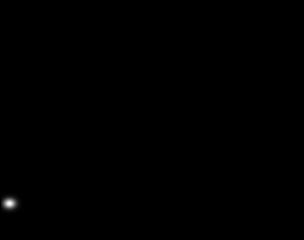
\includegraphics[width=0.23\textwidth]{images/true-field-t=50} & 
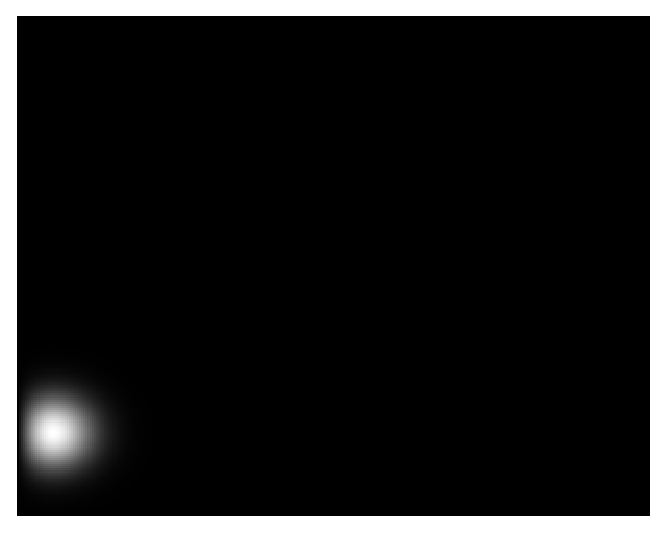
\includegraphics[width=0.23\textwidth]{images/true-field-t=641} &
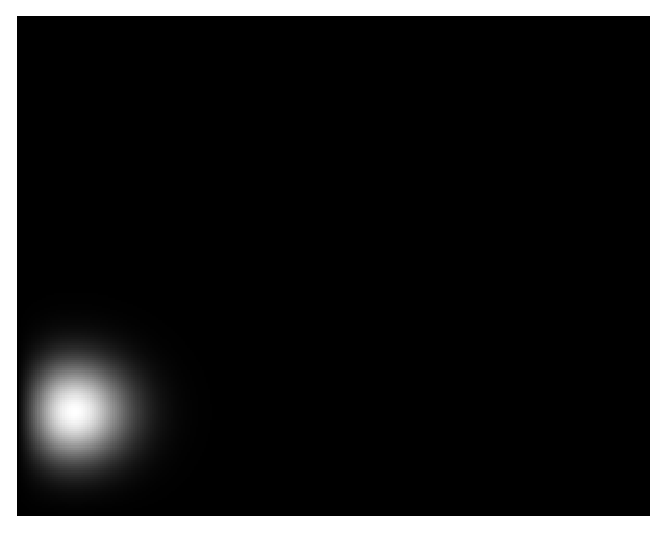
\includegraphics[width=0.23\textwidth]{images/true-field-t=1232} & 
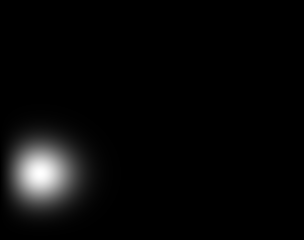
\includegraphics[width=0.23\textwidth]{images/true-field-t=1823} \\
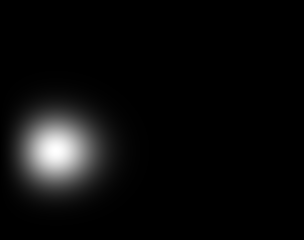
\includegraphics[width=0.23\textwidth]{images/true-field-t=2414} & 
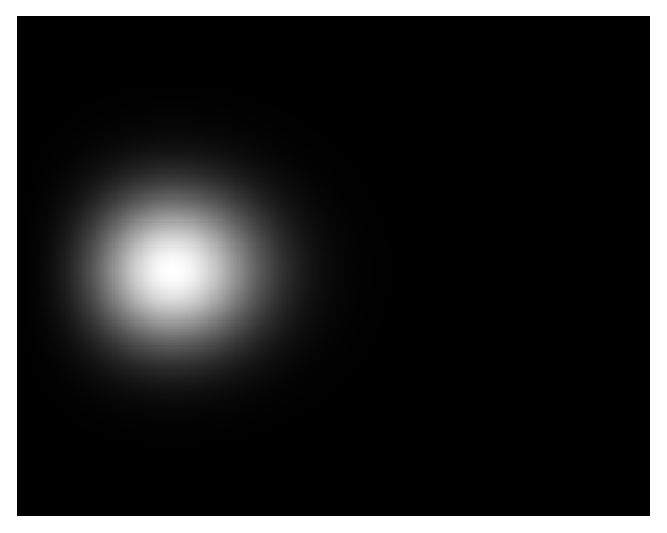
\includegraphics[width=0.23\textwidth]{images/true-field-t=3006} &
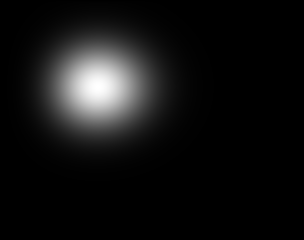
\includegraphics[width=0.23\textwidth]{images/true-field-t=3597} & 
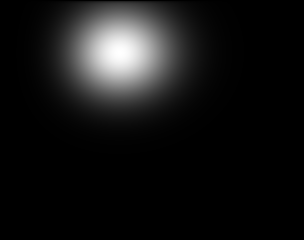
\includegraphics[width=0.23\textwidth]{images/true-field-t=4089} \\
\hline \\
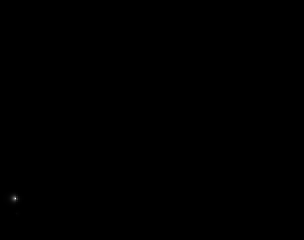
\includegraphics[width=0.23\textwidth]{images/field-t=50} & 
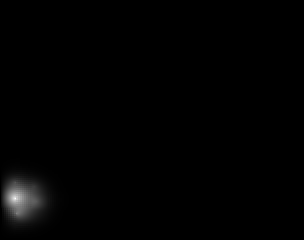
\includegraphics[width=0.23\textwidth]{images/field-t=641} &
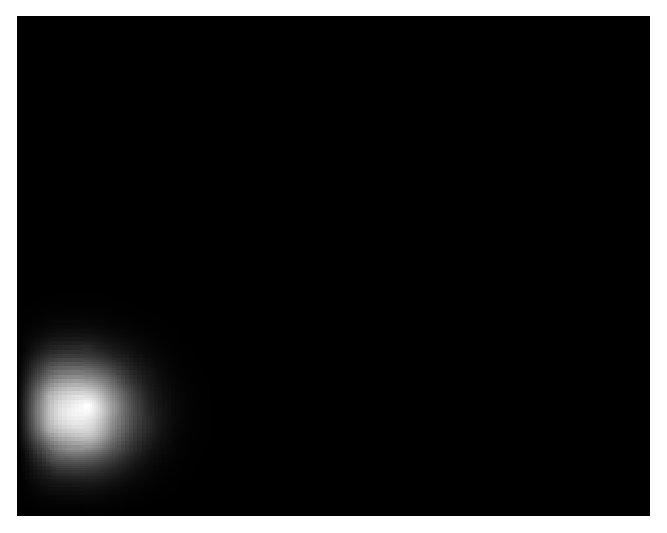
\includegraphics[width=0.23\textwidth]{images/field-t=1232} & 
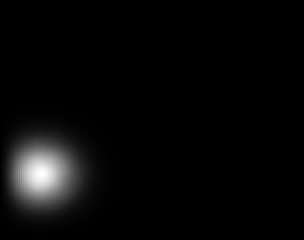
\includegraphics[width=0.23\textwidth]{images/field-t=1823} \\
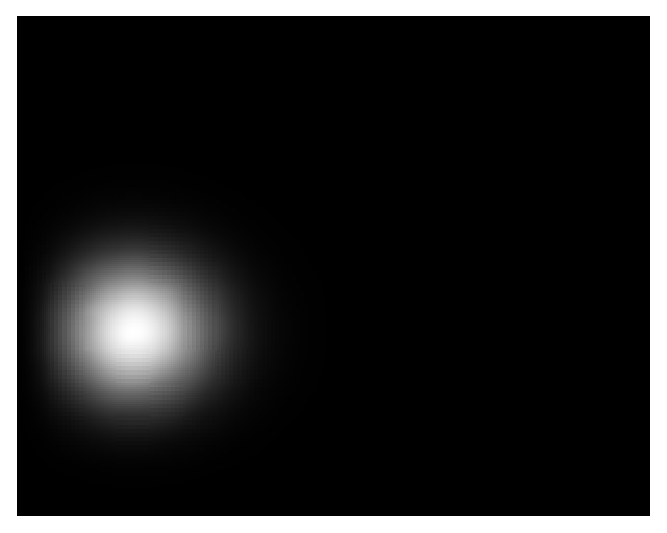
\includegraphics[width=0.23\textwidth]{images/field-t=2414} & 
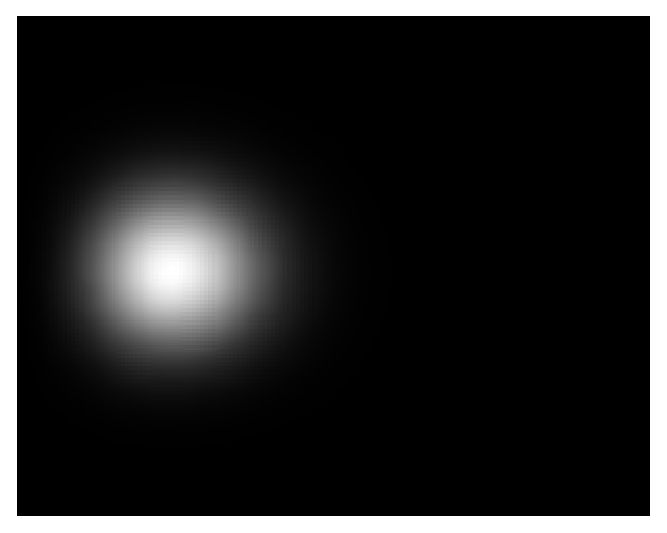
\includegraphics[width=0.23\textwidth]{images/field-t=3006} &
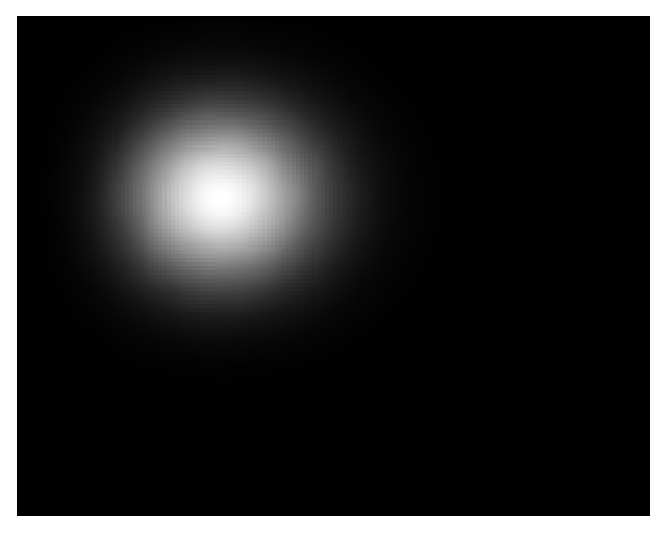
\includegraphics[width=0.23\textwidth]{images/field-t=3597} & 
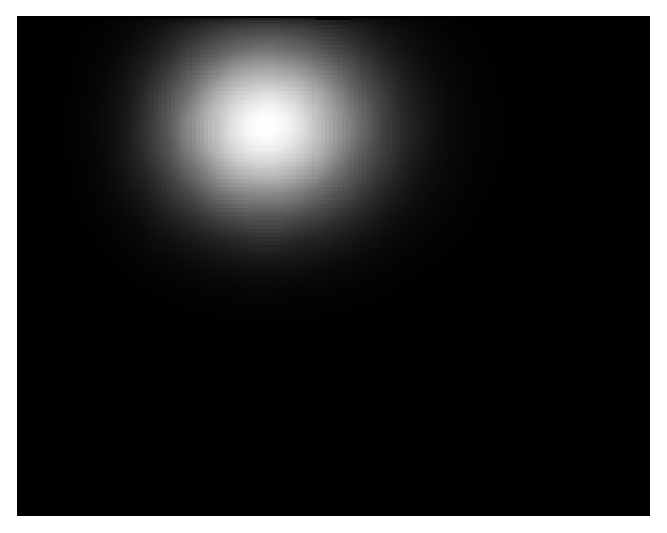
\includegraphics[width=0.23\textwidth]{images/field-t=4089} 
\end{tabular}
\caption{Simulation of advection-diffusion process. \textit{Two top rows} (left to right, then down to left): ground-truth progressing in time. \textit{Two bottom rows} (left to right, then down to left): data-assimilation solution that starts from zero density field and gradually catches up the ground-truth. There are $72960$ nodal points representing $304{\times}240$ domain and $182$ sensors pseudo-randomly scattered therein.}
\label{fig:density}
\end{figure}

Fig.\ref{fig:relerr} shows how relative error fades away as simulation progressing. The relative error is computed as a ratio between $L_2$-norm of flattened field of density difference and  $L_2$-norm of flattened ground-truth density: $\varepsilon$ = $\|u_{gt} - u\|_2/\|u_{gt}\|_2$.

It seems that overall performance of the data-assimilation solver is quite good. It catches up the true distribution as soon as the first sensor has been touched by a high-density spot.  Further improvement would rely on better tuning of Kalman filter by estimating noise covariance matrices directly from data. This is a topic for future research.

\begin{figure}
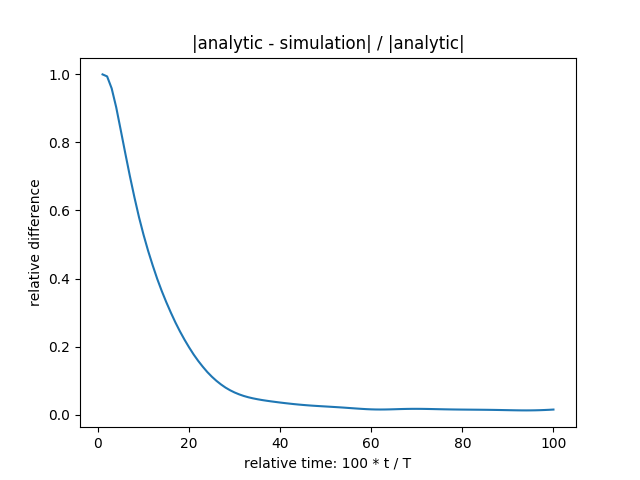
\includegraphics[scale=0.5]{images/rel-diff-Nx304-Ny240}
\caption{Relative difference ($\varepsilon$ = $\|u_{gt} - u\|_2 / \|u_{gt}\|_2$) between the ground-truth density and data-assimilation solution, as a function of ``relative time'': $\tau$ = $100\,t / T$, where $t$ is a physical time in seconds, and $T$ is an integration period.}
\label{fig:relerr}
\end{figure}

Traditionally, the scalability tests are the ones of primal interest in parallel API design. Two tests were conducted in this study on x86 44-core/88-thread machine empowered by Linux RedHat-7.4, 64-bit operating system. In the first test, called ``size scalability'', we enabled all the CPU resources to the application increasing the problem size (number of nodal points in a domain) in a series of simulations. In the second test, called ``multi-threading scalability'', we fixed the problem size increasing the number of working threads from $1$ to $44$ in a series of simulations. Both results are presented on Fig.~\ref{fig:scalability}.

Two important notes should be made at this point. First, the Allscale project is rapidly progressing and in few months the scalability figures will be definitely outdated. Second, one could spot sufficiently long simulation time as can be seen of the left picture of Fig.~\ref{fig:scalability}. As a part of project requirements, we were restricted not to use any optimized libraries for solving a sparse linear system (\ref{eq:state-propag}). Instead, the dense Cholesky and $L U$ solvers had been implemented as a replacement which is accountable for major bottleneck. The end user will not be restricted in such a way, so there should no any concern. 

\begin{figure}
\begin{tabular}{cc}
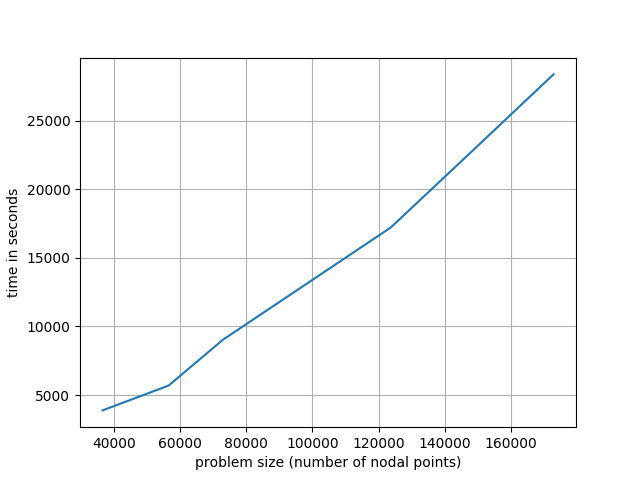
\includegraphics[width=0.48\textwidth]{images/scalability-size} & 
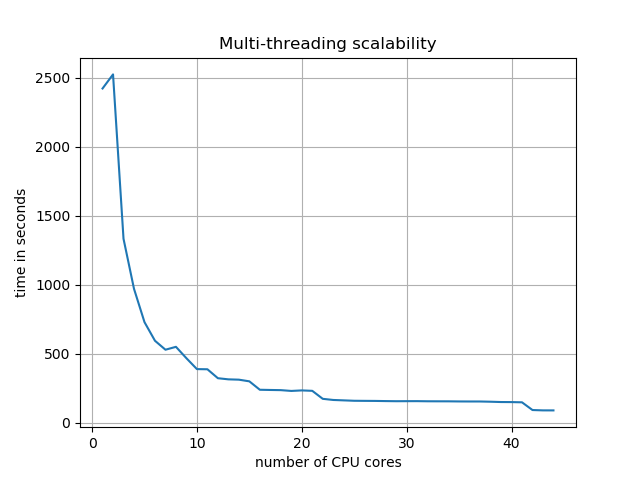
\includegraphics[width=0.48\textwidth]{images/scalability-mt} 
\end{tabular}
\caption{Scalability test results. \textit{Left picture}: size scalability: execution time vs. problem size, all resources are available. \textit{Right picture:} multi-threading scalability: execution time vs. number of working threads.}
\label{fig:scalability}
\end{figure}

%% Acknowledgments
\begin{acks}                            %% acks environment is optional
                                        %% contents suppressed with 'anonymous'
  %% Commands \grantsponsor{<sponsorID>}{<name>}{<url>} and
  %% \grantnum[<url>]{<sponsorID>}{<number>} should be used to
  %% acknowledge financial support and will be used by metadata
  %% extraction tools.
  This material is based upon work supported by the
  \grantsponsor{GS100000001}{National Science
    Foundation}{http://dx.doi.org/10.13039/100000001} under Grant
  No.~\grantnum{GS100000001}{nnnnnnn} and Grant
  No.~\grantnum{GS100000001}{mmmmmmm}.  Any opinions, findings, and
  conclusions or recommendations expressed in this material are those
  of the author and do not necessarily reflect the views of the
  National Science Foundation.
\end{acks}


%% Bibliography
\bibliography{references}


%% Appendix
%\appendix
%\section{Appendix}
%Text of appendix \ldots

\end{document}
